\section{Preliminaries}\label{sec:prel}

This section introduces the basic building blocks of payment channels as well as the original concept of DLC.

\subsection{Transactions}

In Bitcoin a transaction consists of a number of inputs and outputs.
Each output includes a script which specifies under which conditions the ownership of the value contained inside it can be transferred.
Each input refers to a previous output, and needs to provide arguments to satisfy its spending conditions.
Common examples are outputs checking for a digital signature from a specific private key, or requiring signatures from \emph{m} out of \emph{n} possible keys.
Outputs can also contain multiple spending conditions, or spending paths (for example one requiring a single signature, and another one requiring two) that can be created using \Verb_IF/ELSE_ statements.

\subsection{Payment channels}

Payment channels are currently among the most popular solutions to increasing the scalability of blockchain systems.
The concept of payment channels usually revolves around broadcasting a limited number of transactions on the blockchain (called \emph{on-chain} transactions), while enabling a much larger number of transactions to occur.
This can be securely achieved by having two parties exchange transactions and digital signatures in such a way that it is always possible for both of them to enforce the latest state of the channel (the balance between both parties) by broadcasting a transaction \emph{on-chain}, as well as to recover their funds in case their counter party broadcast an outdated state.
A basic assumption for payment channel is that both parties must be watching the blockchain for inclusion of stale transactions, or at least delegate this task to watchtowers~\cite{khabbazian2019}.

\subsection{Transaction revocation}\label{sec:trrev}

In order to protect the parties from the broadcast of an outdated state of the channel, the Lightning Network uses a transaction revocation mechanism.
It works by having both parties hold a different transaction with the same output values, but where the output paying them contains two spending paths:
* The first one requires a signature from a \emph{revocation key},
* The second one requires a signature from the party that holds it, but can only be spent after a certain amount of time has elapsed (using the \Verb_CHECKSEQUENCEVERIFY_ opcode~\cite{csv}).

A party can revoke a transaction by revealing the private key for the first spending path.
If this transaction was to be broadcast \emph{on-chain} in the future, the counter party has a certain amount of time to use the revocation key to claim the funds from the output.
Of course the parties should never reveal their signatures for \emph{their} revokable transactions, as it could allow their counter party to steal their fund if they also know the revocation key.

Note that the protocols and mechanisms for transactions and key exchanges are kept simple in this paper for the purpose of explanation, but the interested reader can refer to the Lightning Network specifications~(\cite{bolt2, bolt3}) for examples of how it can be done in practice.

\subsection{Discreet Log Contracts}\label{basedlc}
DLC were proposed to enable two parties to enter into a financial contract using Bitcoin transactions and an oracle, but without requiring direct interaction with the oracle, thus leaving a “discreet log”.
In other words, the parties do not have to inform the oracle of the contract being established.
This is achieved through a peculiar use of Schnorr signatures~\cite{schnorr1989efficient} that is described in detail in~\cite{dryja2017discreet}.

The second important property of DLC is that they don’t require trust between the parties, and only minimal trust to the oracle (essentially that it does not collude with one of the party).
This is achieved through the use of specially crafted Bitcoin transactions that we recall in this section.
The transaction flow is illustrated in Figure~\ref{fig:basedlc}.

\begin{figure}
  \centering
  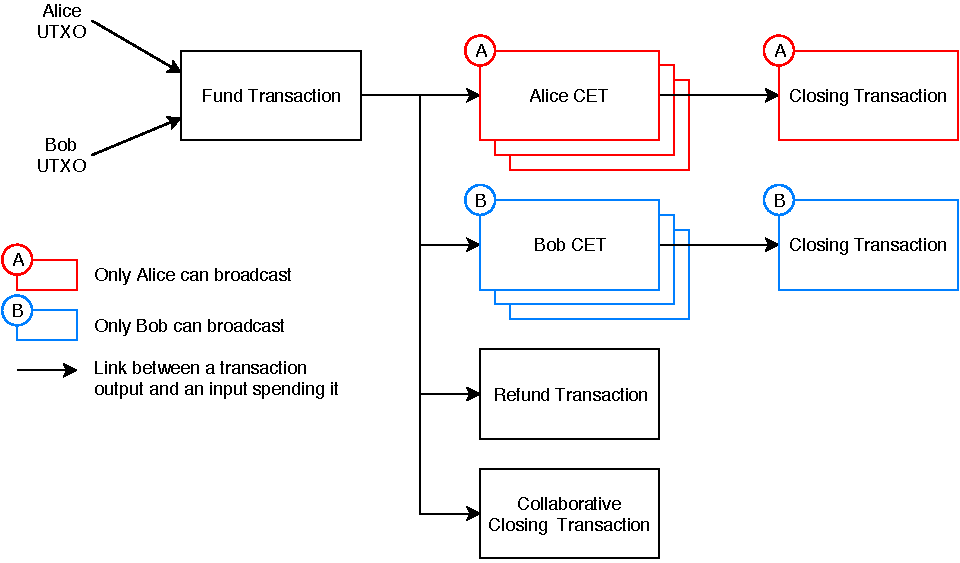
\includegraphics[width=\columnwidth]{Figures/BaseDlc.pdf}
  \caption{Illustration of the on-chain DLC transaction flow. Both parties lock their collaterals in the fund transaction, and can exercise the outcome of the contract through their CETs. Alternatively, the parties can agree to close the contract collaboratively, and if the oracle fails to produce a signature, they can recover their collaterals with the refund transaction.}
  \label{fig:basedlc}
\end{figure}

\subsection{Fund transaction}
The first transaction that makes up a DLC is the fund transaction.
This transaction takes a number of inputs coming from each of the parties UTXOs and locks the collateral of each party into a multi-signature script, requiring a signature from both parties to be unlocked.
It can also include change outputs when the sum of one of the party’s input UTXOs is greater than the desired contract collateral.
The output script for the multi-signature output of the fund transaction is detailed in Script~\ref{script:fundtx}.

\subsection{Refund Transaction}
The refund transaction is one of the transactions that can be used to spend from the fund transaction, and simply returns the collateral posted by each party.
It is intended to be used only in the case where the oracle does not publish a signature for the event on which the DLC is based on.
For that reason, it is time locked, meaning that it cannot be included in the blockchain before a certain timestamp, that should be set to after the maturity date of the contract.

\subsection{Contract Execution Transactions}
A contract execution transaction (CET) is the second type of transaction that can spend from the fund transaction.
It encodes a possible outcome of the contract, meaning that there must be as many CETs as possible outcomes of the contract.
Both parties hold a different set of CETs, each including two outputs.

The first output of a CET consists of a script that enables either the party broadcasting it to spend it by using a combination of its private key and the oracle signature, or their counter party after a certain time has elapsed after the transaction was included in the blockchain (using the Check Sequence Verify op-code \cite{csv}, the script is detailed in Script~\ref{script:cet}).
This ensures that if one of the parties was to broadcast a CET that did not correspond to the outcome revealed by the oracle, they would lose their fund (this is somewhat similar to the transaction revocation concept discussed in Section~\ref{sec:trrev}).

The second output can be spent directly by the counter party of the broadcaster.

\subsection{Closing Transaction}
The closing transaction is used by the broadcaster of a CET to retrieve the funds locked in the first output.
It satisfies the script of the first CET output by providing a signature that is created using a combination of the spender’s private key and the oracle signature.

\subsection{Signing Order}
In order to guarantee that both parties can always either recover their funds or execute the contract, the transactions need to be signed in a specific order. 

First, the signatures for the CETs and the refund transaction are exchanged.
As the fund transaction they spend from has not been signed yet, they cannot be used.

The signatures for the fund transaction are then exchanged.
Note that as this exchange happens non atomically, one of the parties will obtain the other party's signature first.
This gives them a “free option”, in the sense that they can choose to execute the contract only in the event that the outcome is favorable to them.
However, if the counter party does not receive the expected signature, they can choose to spend their UTXOs included in the fund transaction, rendering it invalid, and thus cancelling the contract.

\subsection{Collaborative Closing}

Given the above described transactions, executing a DLC requires broadcasting three transactions: the fund transaction, a CET and a closing transaction.
However, once the Oracle has published the outcome, the parties can decide to create a collaborative closing transaction with the same output amounts as the CET for the announced outcome.
This reduces the number of required transactions to two.
If the parties would like to re-establish a contract after maturity, another two transactions will have to be broadcast \emph{on-chain}.
